\documentclass[10pt, a4paper]{article}
\usepackage{helvet}
\usepackage{amsfonts, amsmath, amssymb}%, amsthm}
\usepackage[none]{hyphenat}
\usepackage{CJKutf8}
\usepackage[T1]{fontenc} % Latin Extended font
\usepackage{ebgaramond} % EB Garamond font
\usepackage{tgheros}    % TeX Gyre Heros font
\usepackage[strict,autostyle]{csquotes} % smart and nestable quote marks
\usepackage[USenglish]{babel} % American English
\usepackage{microtype}% improve text appearance with kerning, etc
\usepackage{datetime} % formatting of date 
\usepackage{tabto}    % make nice tabbing
\usepackage{hyperref} % enable hyperlinks and pdf metadata
\usepackage[top=2cm, bottom=2cm, left=2.5cm, right=2cm]{geometry} % manually set page margins
\usepackage{enumitem} % enumerate with [resume] option
\usepackage{titlesec} % allow custom section fonts
\usepackage{setspace} % custom line spacing
\usepackage{graphicx}
\usepackage{cuted}
\usepackage{caption}
\usepackage{float}
\usepackage{longtable}
\usepackage{hyperref}
\newcommand{\mytitle}{Statistical Pattern Recognition A Review}
\newcommand{\myurl}{https://www.researchgate.net/publication/220181138_Statistical_Pattern_Recognition_A_Review}

\title{Reading Report: \href{\myurl}{\mytitle}}
\author{111C51502, CY Chingyao Fu, NTUT }
\date{Sep 2023}

\begin{document}
\setstretch{1.1}
\begin{CJK*}{UTF8}{bsmi}

\maketitle

\section{Introduction}
五歲的孩子大多數都能識別數字和字母。
圖型識別是研究機器如何觀察環境、學習將感興趣的圖型與其背景區分開來,並判斷圖型。 
儘管經過近50年的研究,通用機器圖型辨識器的設計仍然是一個難以實現的目標。
\subsection{什麼是圖型識別?}
自動(機器)識別、描述、分類和圖型分組是工程和科學學科中的重要議題。例如,圖案可以是指紋圖像、手寫草書字、人臉或語音訊號。 
其識別/分類有兩種: 
(1)Supervised classification(e.g., discriminant analysis),判斷結果為預定義的類別,
(2)Unsupervised classification(e.g., clustering),判斷結果圖型是未知的類別。
\subsection{模板比對}
模板比對是一種最簡單和最早的圖型識別方法。
在模板比對中,使用存儲的模板(通常為2D形狀)或原型,比對要識別的圖型,同時考慮所有的姿態(平移和旋轉)和比例變化。
\subsection{統計分析}
在統計方法中,每個圖型都有 d 個特徵,表示為 d 維空間中的點。 目標是分離佔據 d 維特徵空間中緊湊且不相交區域的特徵。
\subsection{語法分析}
在許多涉及複雜圖型的識別問題中,更適合採用結構化拆分的方式來觀察,其中圖型被視為由相對簡單的子圖型組成,而相對簡單的子圖型本身是由更相對簡單的子圖型建構。
\subsection{神經網路}
神經網路可以被視為大規模平行運算系統,由大量具有許多互連的簡單處理器組成。
神經網路的主要特徵是能夠學習複雜的非線性輸入輸出關係,使用一序列的訓練流程來適應不同的資料。

\section{統計圖像識別}
\begin{figure}[H]
    \centering
    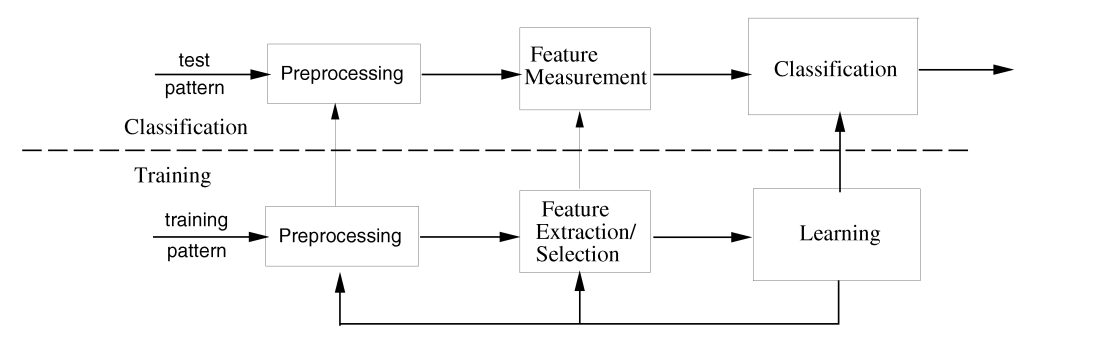
\includegraphics[width=0.9\linewidth]{Model for statistical pattern recognition.PNG}
    \caption{Model for statistical pattern recognition.}
    \label{fig:enter-label}
\end{figure}
在統計圖型辨識中,圖型由一組 d 個特徵表示,被視為 d 維特徵向量。 
利用統計決策理論中的概念來建立圖型類別之間的決策邊界。 
辨識系統以兩種圖型運作:訓練(學習)和分類(測試)。(見Figure 1) \\[0.5em]
預處理模組的作用是從背景中分割感興趣的圖案、去除雜訊、標準化圖案以及有助於定義圖案的緊湊表示的任何其他操作。\\[0.5em]
在訓練圖型中,特徵提取/選擇模組找到用於表示輸入圖型的適當特徵,並且訓練分類器來劃分特徵空間。\\[0.5em]
統計圖型辨識有多種的二分法,見如Figure 2。
統計圖型識別中的大多數方法都使用Bayes Decision Rule。
統計圖型識別中的另一個二分法可以基於決策邊界是直接獲得(幾何方法)或是間接獲得(基於機率密度的方法)。
\begin{figure}[H]
    \centering
    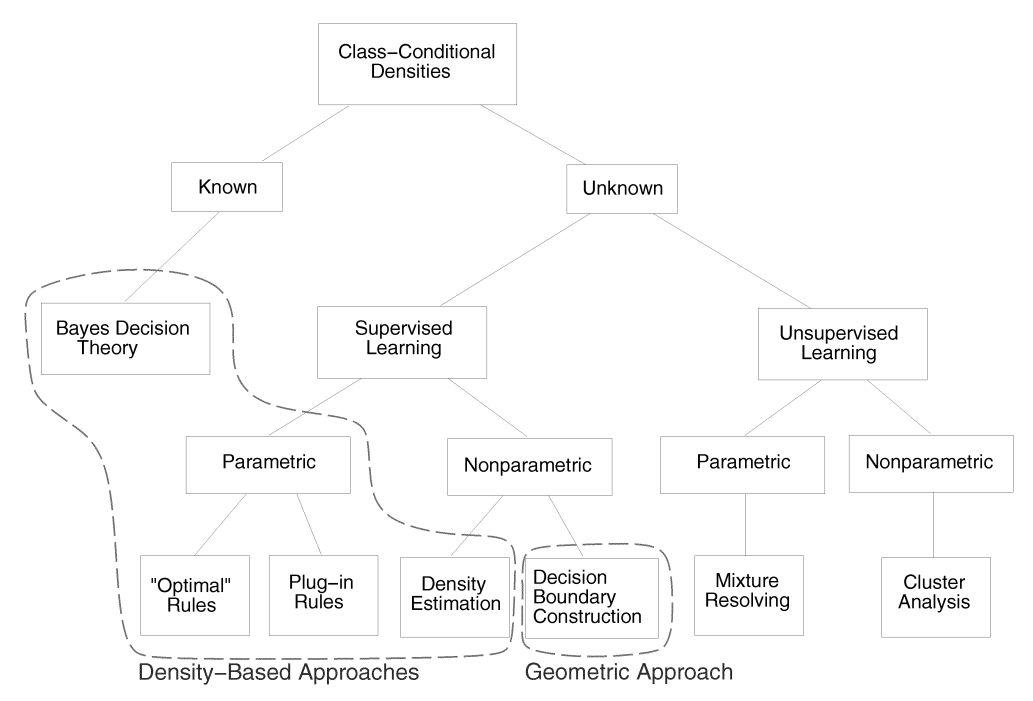
\includegraphics[width=0.9\linewidth]{Various approaches in statistical pattern recognition.PNG}
    \caption{Enter Caption}
    \label{fig:enter-label}
\end{figure}

\section{維度詛咒和峰值現象}
用於機器學習或數據分類的簡單(naive)的表查找(table-lookup)技術,將特徵空間(feature space)劃分成多個單元(cells),然後為每個單元分配一個類標籤(class label)。\\[0.5em]
隨著特徵維度(feature dimension)的增加,特徵空間的大小(即單元的數量)都會倍增,因此需要更多的數據點來填充, 造成訓練數據點(training data points)會呈指數增長。這種現像被稱為“維度詛咒”,導致分類器設計中的“峰值現象”。 \\[0.5em] 
在特定的條件下(1)類條件密度已知(Class-Conditional Densities Are Completely Known),完全理解在每個類別特徵下的概率分佈, (2)訓練樣本數量足夠大和代表性強(Arbitrarily Large and Representative of the Underlying Densities),這些數據點能夠準確地反映每個類別下特徵的真實概率分佈, 增加特徵維度不會導致分類的錯誤率增加。\\[0.5em]
在訓練數據集有限時,應該謹慎選擇特徵,優先考慮最有信息量或最相關的特徵,避免維度詛咒的問題。 \\[0.5em]
在設計分類器時,應確保每個類別(class)的訓練樣本數量(n)應該至少是特徵維度(d)的10倍,有助於緩解過擬合(overfitting)和其他高維數據相關的問題。

\section{降維}
在圖型識別或機器學習中,保持特徵維度盡可能小,可以降低測量成本和提高分類準確度。\\[0.5em]
在訓練樣本數量有限的情況下,減少特徵數量(維度)可以避免維度詛咒問題的影響。\\[0.5em]
特徵選擇(Feature Selection)和特徵提取(Feature Extraction)在圖型識別和機器學習中的不同影響和考慮因素。特徵選擇通常更易於理解和解釋,並且可以減少測量成本。但特徵提取可能會產生具有更強區分能力的新特徵,不過這些新特徵可能缺乏清晰的物理意義。
\subsection{特徵提取}
線性變換的方法,如主成分分析(Principal Component Analysis, PCA)、因子分析(Factor Analysis)、線性判別分析(Linear Discriminant Analysis)和投影追蹤(Projection Pursuit)等,已廣泛應用於圖型識別中的特徵提取和降維。 \\[0.5em]
最廣泛使用是主成分分析PCA或Karhunen-LoeÁve擴展,其捕捉了數據中最主要的變異性,並用於降低數據的維度,同時保留最重要的信息。\\[0.5em]
投影追蹤 (Projection Pursuit)和獨立成分分析(Independent Component Analysis, ICA)特別適用於非高斯分佈的數據,因為它們不依賴於數據的均值和方差,而能夠捕捉數據中更複雜的結構和相關性。
\subsection{特徵選擇}
近年來,由於(1)多感測器融合(Multisensor Fusion):來自多個感測器的數據會被合併,導致特徵數量大幅增加。(2)多數據模型的整合(Integration of Multiple Data Models):當多個數據模型或來源被結合在一起時,特徵的數量和複雜性也會增加,因此特徵選擇變得特別重要。可以幫助減少計算成本,提高模型的準確性和可解釋性。\\[0.5em]
Cover和Van Campenhout的研究結果表明:沒有非窮舉(nonexhaustive)的順序特徵選擇(sequential feature selection)程序可以保證產生最優的特徵子集。即非窮舉的順序特徵選擇方法不能保證找到最佳解。\\[0.5em]
唯一能夠在避免窮舉搜索的情況下達到"最優"(根據一類單調標準函數)的特徵選擇方法是基於分支界定(Branch and Bound)算法。

\section{分類器}
最基本的分類器是根據數據點之間的相似性(concept of similarity)來進行分類。\\[0.5em]
貝葉斯決策規則(optimal Bayes decision rule)是基於概率的,以後驗概率(posterior probability)做爲判斷。\\[0.5em]
1-NN(1-Nearest Neighbor)是一個簡單但有效的分類器,常用作其他更複雜分類器的比較基準。\\[0.5em]
第三類分類器不是基於相似性或概率,而是通過最小化錯誤(error criterion)來找到最佳的決策邊界。\\[0.5em]
支持向量機(Support Vector Classifier, SVC)可以看作是一種高級形式的模板匹配(template matching),但它更注重找到最優的決策邊界。\\[0.5em]
決策樹(Decision Tree)是一簡單但強大的分類器,它在每一步都選擇最重要的特徵進行區分。\\[0.5em]
神經網絡(Multilayer Perceptrons, MLP)能夠捕捉複雜的非線性關係,但如果模型太複雜,可能會導致overtraining。\\[0.5em]
SVM(Support Vector Classifier)是非常高效的,特別是在高維數據和有限的訓練樣本中。\\[0.5em]
沒有一種分類器(classifier)是在所有情況下都是最好的,選擇哪種分類器取決於具體的應用場景。\\[0.5em]
\begin{longtable}{| p{4.5cm} | p{10cm} |}
    \caption{Classification Methods} \\
    \hline
    方法 (Method) & 屬性 (Property) \\
    \hline
    \endfirsthead
    Template matching & 將樣本分配給最相似的模板。 \\
    \hline
    Nearest Mean Classifier & 將樣本分配給最近的類均值。 \\
    \hline
    Subspace Method & 將樣本分配給最近的類子空間。 \\
    \hline
    1-NN (1-Nearest Neighbor Rule) & 將樣本分配給最近訓練樣本的類。 \\
    \hline
    k-NN (k-Nearest Neighbor Rule) & 根據k個最近鄰居中性能最佳的k值,將樣本分配給多數類。 \\
    \hline
    Bayes plug-in & 將樣本分配給具有最大估計後驗概率的類。 \\
    \hline
    Logistic Classifier & 最大似然規則用於羅吉斯(S型)後驗概率。 \\
    \hline
    Parzen Classifier & 用於Parzen密度估計的Bayes plug-in,具有性能最佳化的內核。 \\
    \hline
    Fisher Linear Discriminant & 使用均方誤差優化的線性分類器。 \\
    \hline
    Binary Decision Tree & 找到一組用於圖案相關特徵序列的閾值。 \\
    \hline
    Perceptron & 線性分類器的迭代優化。 \\
    \hline
    Multi-layer Perceptron & 使用S型傳遞函數對兩層或更多層的感知器(神經元)進行均方誤差的迭代優化。 \\
    \hline
    Radial Basis Network & 對具有至少一層使用高斯型傳遞函數的神經元的前馈神經網絡進行均方誤差的迭代優化。 \\
    \hline
    Support Vector Classifier & 通過選擇最少數量的支持向量來最大化類之間的邊界。 \\
    \hline
\end{longtable}

\section{分類器組合}
解決分類問題時,可能會結合多個分類器,原因包含:多元表示/描述 (Different Representations), 多個訓練集 (Multiple Training Sets), 局部差異 (Local Differences), 隨機初始化 (Random Initialization)。\\[0.5em]
結合方案 (Combination Schemes)則有: 并聯結構 (Parallel), 串聯結構 (Cascading or Serial), 層次結構 (Hierarchical)。
\subsection{單獨分類器的選擇和訓練}
分類器組合(Classifier Combination)特別有用,其中每個分類器(Individual Classifiers)基本是獨立的。\\[0.5em]
獨立的分類器會具有幾個優點:多樣性(Diversity), 錯誤糾正(Error Correction), 泛化能力(Generalization), 計算效率(Computational Efficiency)
\subsection{組合器(Combiner)}
在選擇了數個單個分類器(Individual Classifiers)後,需要通過組合器(Combiner)的模塊將它們組合在一起。組合器有多種,它們在可訓練性(Trainability)、適應性(Adaptivity)和對單個分類器輸出的需求方面有所不同。
\subsection{組合方案分析}
分類器組合在實驗研究中已經被證明是有效的,可以提高模型的識別能力。\\[0.5em]
回歸或分類錯誤可以分解為偏差項(Bias Term)和方差項(Variance Term), 這是評估分類器性能的一個重要參數。\\[0.5em]
N個Unbiased Neural Networks的線性組合,具有independent and identically distributed (i.i.d.)的誤差分佈,可以將方差減少N倍。\\[0.5em]
Sum Rule是當需要組合相同後驗概率的不同估計時最適合的。\\[0.5em]
泛化錯誤(Generalization Error)受到訓練數據上邊界分佈(Margin Distribution)的尾部概率以及單個分類器(Single Classifier)複雜度的函數所影響,不僅取決於組合分類器,還取決於單個分類器的複雜度。

\section{誤差估計}
錯誤率(Error Rate)是用來評估分類器是否有效的最終衡量標準。它表示分類器做出錯誤判斷的頻率。\\[0.5em]
分類器首先使用訓練樣本來設計,然後使用測試樣本來評估其性能。
同時,訓練和測試樣本必須是獨立的,以確保模型的泛化能力。\\[0.5em]
每個測試樣本都有兩種可能的結果:被正確分類或被錯誤分類,其遵循二項分佈(Binomial Distribution)的統計原則。\\[0.5em]
常見的進階性能指標:偽接受率(False Acceptance Rate, FAR)和偽拒絕率(False Reject Rate, FRR), FAR對FRR的繪圖稱爲"接收操作特性曲線"(Receiver Operating Characteristic, ROC Curve), 拒絕率(Reject Rate)。

\section{非監督式分類}
非監督分類(Unsupervised Classification)是一種機器學習方法,其中訓練數據沒有標籤。目標是根據這些未標籤的數據來建立決策邊界。\\[0.5em]
數據聚類(Data Clustering)是非監督分類的另一種稱呼,主要目的是在多維數據中找到自然的分組或聚類。聚類分析是一個非常重要和有用的技術。但是,它也有其挑戰,例如選擇合適的相似性度量、確定聚類的數量等。\\[0.5em]
大多數聚類算法基於兩種流行的聚類技術:迭代平方誤差劃分聚類(Iterative Square-error Partitional Clustering)和凝聚層次聚類(Agglomerative Hierarchical Clustering)。
\subsection{平方誤差聚類(Square-Error Clustering)}
平方誤差分類是最常用的聚類策略。其主要目的是在固定數量的聚類下,找到最小化平方誤差的方法。\\[0.5em]
K-均值算法(K-means Algorithm)是平方誤差分類的一個特例,采用迭代的劃分聚類方法,將數據點分配到K個不同的聚類中,使每個數據點都屬於與其最近的中心(均值)的聚類。\\[0.5em]
聚類的一個主要挑戰是缺乏選擇K值、初始劃分、更新劃分、調整聚類數量和停止標準的標準。\\[0.5em]
為了提高基本K-均值算法的性能,已經有多種嘗試,包括加入模糊標準函數(Fuzzy Criterion Function)、使用遺傳算法(Genetic Algorithms)、模擬退火(Simulated Annealing)和禁忌搜索(Tabu Search)來優化結果劃分。\\[0.5em]
向量量化(Vector Quantization)可以視為一種聚類的問題,將高維數據(例如,聲音或圖像)編碼為低維符號的技術,這些低維符號通常來自一個稱為"輸出字母表"(Output Alphabet)的有限集合, 將向量量化問題轉化為聚類問題,從而可以利用聚類算法(如K-均值)來解決向量量化問題。
\subsection{混合物分解(Mixture Decomposition)}
混合模型(Mixtures)的主要用途是用來定義無監督分類(Unsupervised Classification),混合模型能夠捕捉到數據可能來自多個不同來源的特性,這使它們在無監督分類中特別有用。\\[0.5em]
混合模型(Mixtures)也非常適合於監督學習場景(Supervised Learning Scenarios)中表示複雜的類條件密度(Class-Conditional Densities)。
\subsubsection{基本定義}
考慮一種生成隨機樣本的方法,其中有K個不同的隨機來源,每個來源都有一個特定的概率分佈。這種生成機制產生的隨機變數遵循一個有限混合分佈(Finite Mixture Distribution),這個分佈是所有來源分佈的加權和。\\[0.5em]
混合擬合需要解決兩個問題, 一是如何找出每個來源的概率分佈,二是有多少個不同的來源。一般使用期望最大化(Expectation-Maximization, EM)算法來估計這些參數。
\subsubsection{EM Algorithm}
EM算法假設我們有一些觀察數據,但這些數據缺少一些信息(標籤),這些信息是我們需要估計的。\\[0.5em]
EM算法主要由兩個步驟組成。E步驟用於估計缺失數據,而M步驟則用於更新模型參數。\\[0.5em]
使用EM進行混合模型(mixture model)擬合的主要困難是:它的局部性質使其嚴重依賴於初始化;還有可能收斂到參數空間的邊界點。
\subsubsection{估計成分數量}
最大似然(ML, Maximum Likelihood)方法在混合模型(Mixture Models)中不能單獨用來確定群集Cluster的數量(K)。因爲當增加K值時,模型會變得更靈活,能更好地擬合數據,從而導致似然性(Likelihood)也會增加,造成Overfitting,失去泛化能力。\\[0.5em]
因此,可以使用一個成本函數(Cost Function)來評估模型, 一方面考慮模型對數據的擬合度(通常用似然性來衡量);一方面考慮模型複雜度(通常用K值來衡量,因為K值越大,模型越複雜)。找到一個能使成本函數最小化的K值。這個K值應該能達到模型複雜度和擬合度之間的最佳平衡。

\section{討論}
圖案識別(Pattern Recognition)領域的前沿主題和研究方向。以下是幾個主要的重點:
\begin{itemize}
  \item 模型選擇(Model Selection):為了避免維度詛咒(Curse of Dimensionality),模型選擇一直是研究的熱點。常用的方法包括Cross-validation和Bayesian Methods。
  \item 混合模型和EM算法(Mixture Modeling and EM Algorithm):這是一種用於密度估計和聚類的流行方法。
  \item 支持向量機(SVM)和結構風險最小化(Structural Risk Minimization):SVM基於結構風險最小化理論,已經在多個應用中展示了其優越性。
  \item 局部決策邊界學習(Local Decision Boundary Learning):這主要是使用不同類別邊界附近的圖案來構建或修改決策邊界。
  \item 順序圖案識別(Sequential Pattern Recognition):隱馬爾可夫模型(Hidden Markov Models, HMM)是一個流行的工具,用於模型和識別順序數據。
  \item 數據壓縮和分類準確性(Data Compression and Classification Accuracy):使用空間和頻譜相關性或馬爾可夫結構來壓縮數據。
  \item 半監督學習(Semi-supervised Learning):如何使用未標籤的數據進行訓練是一個重要問題。
  \item 不變圖案識別(Invariant Pattern Recognition):這在字符和臉部識別等多個應用中是可取的。
  \item 上下文信息的使用(Use of Contextual Information):這在語音識別、光學字符識別(OCR)和遙感等方面已經成功地使用。
\end{itemize}

\end{CJK*}
\end{document}
